% This is the file where my Master Thesis will be written. It uses the adapted
% LNCS Template.
%
% I'll be using a few codes in the comments, which can be easily looked up:
% * NOTE: theseis-text related comments
% * TODO: thesis-related TODO's
% * WARN: latex/formatting-related warningss
%
% WARN: for running head, subsititute the line below by:
% \documentclass[runningheads,a4paper]{llncs}
\documentclass{llncs}

%\usepackage{geometry}

%\geometry{
%a4paper,         % or letterpaper
%textwidth=12.9cm,  % llncs has 12.2cm
%textheight=19.9cm, % llncs has 19.3cm
%heightrounded,   % integer number of lines
%hratio=1:1,      % horizontally centered
%vratio=2:3,      % not vertically centered
%}
%
%%% WARN: custom extension
\usepackage{xcolor}
\newcommand{\todo}[1]{\textcolor{red}{TODO: #1}\PackageWarning{TODO:}{#1!}}

%%% GLOSSARIES
\usepackage{glossaries}

%%% inline code
\usepackage{xparse}
\NewDocumentCommand{\codeword}{v}{%
\texttt{\textcolor{blue}{#1}}%
}

%%% figures
\usepackage{graphicx}
\usepackage{wrapfig}

%%% tables
\usepackage{booktabs}

\usepackage{amssymb}

\usepackage{url}
\def\UrlBreaks{\do\/\do-}


\makeglossaries

\newacronym{tls}{TLS}{Transport Layer Security}%
\newacronym{ssl}{SSL}{Secure Sockets Layer}%
\newacronym{ietf}{IETF}{Internet Engineering Task Force}%
\newacronym{mac}{MAC}{Message Authentication Code}%
\newacronym{psk}{PSK}{Pre-Shared Key}%
\newacronym{rpk}{RPK}{Raw Public Key}%
\newacronym{aead}{AEAD}{Authenticated Encryption With Associated Data}%
\newacronym{pkc}{PKC}{Public Key Cryptography}%
\newacronym{hkdf}{HKDF}{HMAC-based Extract-and-Expand Key Derivation Function}%
\newacronym{html}{HTML}{Hypertext Markup Language}%
\newacronym{https}{HTTPS}{Hypertext Transfer Protocol Secure}%
\newacronym{ecc}{ECC}{Elliptic Curve Cryptography}%
\newacronym{iv}{IV}{Initialization Vector}%
\newacronym{ecdh}{ECDH}{Elliptic Curve Diffie-Hellman}%
\newacronym{ecdhe}{ECDHE}{Elliptic Curve Diffie-Hellman Ephemeral}%
\newacronym{ecdsa}{ECDSA}{Elliptic Curve Digital Signature Algorithm}%
\newacronym{rfc}{RFC}{Request For Comment}%
\newacronym{prf}{PRF}{Pseudo-Random Function}%
\newacronym{rsa}{RSA}{Rivest-Shamir-Adleman}%
\newacronym{dh}{DH}{Diffie-Hellman}%
\newacronym{pms}{PMS}{premaster secret}%
\newacronym{dsa}{DSA}{Digital Signature Algorithm}%
\newacronym{pfs}{PFS}{Perfect Forward Secrecy}%
\newacronym{mitm}{MITM}{Man In The Middle}%
\newacronym{ac}{AC}{Asymmetrical Cryptography}%
\newacronym{sc}{SC}{Symmetrical Cryptography}%
\newacronym{iot}{IoT}{Internet Of Things}%
\newacronym{dtls}{DTLS}{Datagram TLS}%
\newacronym{coap}{CoAP}{Constrained Application Protocol}%
\newacronym{ec}{EC}{Elliptic Curve}%
\newacronym{sca}{SCA}{Side-Channel Attack}%
\newacronym{ocsp}{OCSP}{Online Certificate Status Protocol}
\newacronym{crl}{CRL}{Certificate Revocation List}
\newacronym{ca}{CA}{Certification Authority}
\newacronym{sni}{SNI}{Server Name Indication}
\newacronym{dos}{DoS}{Denial-of-Service}
\newacronym{ddos}{DDoS}{Distributed Denial-Of-Service}
\newacronym{pki}{PKI}{Public Key Infrastructure}
\newacronym{ae}{AE}{Authenticated Encryption}
\newacronym{nsa}{NSA}{US National Security Agency}
\newacronym{apk}{APK}{Authorized Public Key}


%%% WARN: added as specified here:
% https://tex.stackexchange.com/questions/272200/table-of-contents-showing-the-title-as-only-entry-latex
\setcounter{tocdepth}{2}
\makeatletter
\renewcommand*\l@author[2]{} % removes author name from TOC
\renewcommand*\l@title[2]{} % removes title name from TOC
\makeatletter
%%%
%
\usepackage{makeidx}  % allows for indexgeneration
%
\begin{document}
%
\frontmatter          % for the preliminaries
%
\pagestyle{headings}  % switches on printing of running heads
%
\addtocmark{TLS For IoT} % additional mark in the TOC

\tableofcontents
\newpage

\mainmatter              % start of the contributions
%
\title{Transport Layer Security Protocol For Internet Of Things}
%
\titlerunning{TLS For IoT}  % abbreviated title (for running head)
%                                     also used for the TOC unless
%                                     \toctitle is used
%
\author{{Illya Gerasymchuk} \\
\email{illya.gerasymchuk@tecnico.uliboa.pt}
%
\authorrunning{Illya Gerasymchuk} % abbreviated author list (for running head)
%
%%%% list of authors for the TOC (use if author list has to be modified)
\tocauthor{Illya Gerasymchuk}
%
\institute{Instituto Superior Técnico}
% WARN: supper hacked-in
\supervisors{Ricardo Chaves, Aleksandar Ilic}
\maketitle              % typeset the title of the contribution

\begin{abstract}
\gls{tls} is, by far, the most used communication security protocol, it is however, not suitable in the context of \gls{iot}. The resource-limited nature
of a big part of \gls{iot} devices does not allow for the use of computationally complex
and memory demanding operations present in a standard \gls{tls} implementation. Most of previous work focused entirely on \gls{dtls} and
can not be easily integrated with existing deployments. This work focuses on
how \gls{tls} and the extension mechanism can be used to define a framework
to adapt the protocol to specific needs. This is the approach that
will be followed in the second part of the work. Having an adaptable and
easy to use solution is crucial for its adaptation in \gls{iot},
where security might have been completely foregone otherwise.

\keywords{TLS, DTLS, SSL, IoT, cryptography, protocol, lightweight cryptography}
\end{abstract}
%
\section{Intoduction}
%

The Internet of Things (IoT) is a network of devices, from simple sensors to smartphones and wearables
which are connected together. In fact, it can be any other object that has an assigned
IP address and is provided with the ability to transfer data over a network. Even a salt shaker\cite{SMALTThe76:online} can now be part of the global network.

The \gls{iot} technology provides many benefits, from personal comfort to
transforming entire industries, mainly due to increased connectivity and
new sources for data analysis. The technological development, however, tends to focus on
innovative design rather than on privacy and security. \gls{iot} devices frequently
connect to networks using inadequate security and are hard to update when
vulnerabilities are found.

This lack of security in the \gls{iot} ecosystem has been exploited by the
the \textit{Mirai} botnet\cite{sec17ant94:online} when it overwhelmed several high-profile
targets with massive \gls{ddos} attacks. This is the most devastating attack involving \gls{iot}
devices done to date. However, the \textit{Reaper} botnet\cite{ReaperCa10:online} could be
even worse if it is ever put to malicious use. Similar attacks will inadvertently
come in the future.

\gls{tls} is one of the most used security protocols in the world, allowing two peers
to communicate securely. It is designed to run on top of a reliable, connection-oriented
protocol, such as TCP. Datagram TLS (DTLS) is the version of \gls{tls} that runs on top
of an unreliable transport protocol, such as UDP. Most \gls{iot} devices have
very limited processing power, storage and energy. Moreover, the performance of
TCP is known to be inefficient in wireless networks, due to its congestion control
algorithm. This situation is worsened with the use of low-power radios and lossy
links found in sensor networks. Therefore, the use of TCP with \gls{iot}
is usually not the best option. For this reason, \gls{dtls}, which runs on top
of UDP, is used more frequently in such devices. The work that will be done in the context of this dissertation, can however,
be applied to either one of them, so even though mostly
\gls{tls} will be mentioned, almost everything can also be applied to \gls{dtls}. This is a consequence of \gls{dtls} being just an adaption of \gls{tls} over unreliable transport protocols, with no changes done to
the core protocol.

The problem in using (D)\gls{tls} in \gls{iot} is that it is not lightweight, since
it has not been designed for such environments. An \gls{iot} device may only have
$256$ KB of RAM and needs to conserve the battery, while sending and receiving
a large amount of small information constantly. For example, consider the case of a temperature sensor
that sends temperature measures every $30$ seconds to a server. In this case
it just needs to send a few bytes of data and do it with minimal overhead, to conserve
RAM and battery. If that sensor is going to use (D)\gls{tls} $1.2$, it will need
two extra roundtrips before it can send any data. This can result in an overhead of several hundreds of
milliseconds. Besides that, it will need to perform heavy mathematical operations
involved in cryptography, using even more energy and taking even more time.
Given this, there is a clear need for a more lightweight (D)\gls{tls} for the \gls{iot}.

The goal of this work is to develop a lightweight version of (D)\gls{tls} that is
fully backwards compatible and does not require any third-party entities, in order
to simplify its deployment process. The solution will be developed for
(D)\gls{tls} version $1.2$, while also bearing in mind the new $1.3$ version. The idea is to make it customizable,
depending on the security requirements and the context of its usage.

In the process of the work on this dissertation, we have already made several
contributions to the \gls{tls} $1.3$ specification, being recognized as contributors\cite{Mergepul65:online}.

The document is organized as follows: Section 2 describes the background. It
introduces some of the concepts that will be used throughout
the document. Section 3 describes the \gls{tls} and \gls{dtls} protocol
versions $1.2$ and $1.3$, with a focus on the version $1.2$ since
it is the latest and the most used version of the protocol (version $1.3$ is still in
draft mode). Section 4 describes all of the related work done in the area and
the current state of the art. Section 5 provides an architecture of the
solution that will be developed in the second part of the dissertation,
and describes how the results will be evaluated and presents a general work plan. Finally, the conclusion of the work is done in Section 6.

\section{Background}

\gls{tls} is a complex protocol that relies on various concepts to provide
security. The most relevant ones will be described here.

In a typical scenario, \gls{tls} uses \gls{ac} for peer authentication and \gls{sc} for bulk data
encryption and integrity protection, for this reason this topic will be covered in Section \ref{sac}. Section \ref{pccc} covers the most common way of peer authentication: public key certificates. Authenticated Encryption With Additional Data (AEAD) ciphers offer various advantages in the
context of \gls{iot}, particularly less computational and spacial overhead.
Furthermore, they are the only type of ciphers that can be used in \gls{tls}
$1.3$. For those reasons, they're covered in Section \ref{aeadciphers}.
When compared to other public key cryptography approaches, \gls{ecc} offers shorter keys, lower processing requirements and lower memory usage for equivalent security strength, being heavily used
in \gls{tls}. An overview of \gls{ecc} in presented in Section \ref{eccsection}.


\subsection{Symmetric vs Asymmetric Cryptography} \label{sac}

\gls{ac} is more expensive than \gls{sc} in terms of performance. There are two main reasons for this. First, larger key sizes are required for an \gls{ac} system to achieve the
same level of security as in a \gls{sc} system. Second, \codeword{CPU}s are slower at performing the underlying
mathematical operations involved in \gls{ac}, namely exponentiation requires
$O(log e)$ multiplications for an exponent $e$. The 2016 \codeword{NIST} report \cite{Recommen44:online}
suggests that an \gls{ac} algorithm would need to use a secret key with size of \codeword{15360 bits}
to have equivalent security to a \codeword{256-bit} secret key for a \gls{sc} algorithm.
This situation is ameliorated by \gls{ecc}, which requires keys of \codeword{512 bits}, but
it is still slower than using \gls{sc}. The 2017 \codeword{BSI} report \cite{Kryptogr1:online} (from the
German federal office for information security) suggests similar numbers.

Another argument for avoiding the use of \gls{ac}
algorithms as much as possible, is that they require additional storage space. This can be a problem for many \gls{iot} devices,
like \codeword{class 1} devices according to the terminology of constrained-code
networks\cite{RFC7228} which have approximately \codeword{10KB} of RAM and \codeword{100KB}
of persistent memory. We measured and compared the resulting size of the \textit{mbedTLS 2.6.0} library\cite{SSLLibra13:online} binary when it was compiled with and without the \gls{rsa} module
(located in the \codeword{rsa.c} file). The conclusion is that that using the \codeword{rsa.c} module adds an overhead of about \codeword{32KB}.

\subsection{Public Certificates and Certificate Chains} \label{pccc}

A public key certificate, also known as a digital certificate, is an electronic
document used to prove the ownership of a public key. This allows other parties
to rely upon assertions made by the private key that corresponds to the public key
that is certified. In the context of (D)\gls{tls}, certificates serve as a guarantee
that the communication is done with the claimed entity and not someone impersonating it.

A \gls{ca} is an entity that issues digital certificates. There are two types of
\gls{ca}s: the \textbf{root \gls{ca}s} and the \textbf{intermediate \gls{ca}s}.
An intermediate \gls{ca} is provided with a certificate with signing capabilities
signed by one of the root \gls{ca}s. A \textbf{certificate chain} is a list of
certificates from the root certificate to the end-user certificate, including
any intermediate certificates along the way. In order for a certificate
to be trusted by a device, it must be directly or indirectly issued by a \gls{ca} trusted by the device.

In (D)\gls{tls}, the certificates are in the \codeword{X.509} format, defined
in \codeword{RFC 5280}\cite{rfc5280}.

\subsection{\gls{aead} Ciphers} \label{aeadciphers}

\gls{ae} and \gls{aead} are forms of encryption which simultaneously provide
confidentiality, integrity and authenticity guarantees on the data. An \gls{ae}
cipher takes as input a \codeword{key}, a \codeword{nonce} and a \codeword{plaintext}
and outputs the pair \codeword{(ciphertext, MAC)}, if it is encrypting and does the inverse
process, while also performing the \gls{mac} check if it is decrypting.

\gls{aead} is nothing more than a variant of \gls{ae}, which comes with an extra
input parameter that is additional data, that is \textbf{only authenticated, but not encrypted}.
Some \gls{aead} ciphers have shorter authentication tags (\textit{i.e.} shorter \gls{mac}s),
which makes then more suitable for low-bandwidth networks, since the messages to be sent are smaller in size.

\subsection{\gls{ecc}} \label{eccsection}

public key cryptography is based on the use of one-way math functions. Such
functions make it easy to compute the answer given an input,
but hard to compute the input given the answer. For example, RSA uses factoring
as the one one way function: it is easy to multiply large numbers, but it is hard
to factor them.

\gls{ecc} is based on elliptic curves, which are set of points $(x,y)$ that are
solutions to the equation $y^2 = x^3 + ax + b$, where $4a^3 + 27b^2 \neq 0$.
Depending on the value of $a$ and $b$, elliptic curves assume different shapes
on the plane.

The security of \gls{ecc} is based on the elliptic curve discrete logarithm
problem. It states that scalar multiplication is a one way function. To exemplify,
given a curve $E(\mathbb{Z}/p\mathbb{Z})$ and points $Q$ and $P$ on that curve
$Q,P \in E(\mathbb{Z}/p\mathbb{Z})$, where $Q$ is a multiple of $P$, the elliptic curve discrete logarithm problem
states that finding the integer $k$, such that $Q=kP$ is a very hard problem.

\section{The \gls{tls} Protocol}

\gls{tls} is a \textbf{client-server} protocol
that runs on top a \textbf{connection-oriented and reliable transport protocol},
such as \textbf{TCP}. Its main goal is to provide \textbf{privacy} and \textbf{integrity}
between the two communicating peers. Privacy implies that a third party will not
be able to read the data, while integrity means that a third party will not be
able to alter the data.

In the TCP/IP Protocol Stack, \gls{tls} is placed between the \textbf{Transport}
and \textbf{Application} layers. It is designed to simplify the establishment
and use of secure communications from the application developer's standpoint.
The developer's task is reduced to creating a "secure" connection (\textit{i.e.} socket), instead of a "normal" one.

A secure communication established using \gls{tls} has two phases. In the first
phase, the communicating peers authenticate one to another and negotiate the parameters, such as the secret keys and the encryption algorithm. In the
second phase, they exchange cryptographically protected data under
the previously negotiated parameters. The first phase is done under the
Handshke Protocol and the second under the Record Protocol. In order to
achieve its goals, during the Handshake Protocol the client and the server
exchange various messages. The message flow is depicted in Figure \ref{fig:tls-12-handshake} and described in more detail in Section
\ref{hsp}.

\gls{tls} provides the following \textbf{security services}:
\begin{itemize}
\item \textbf{authentication} - both, \textbf{peer entity} and \textbf{data origin} (or \textbf{integrity})
authentication.
\subitem \textbf{peer entity authentication} - a peer has a guarantee that it is talking to certain entity, for example, \codeword{www.google.com}.
This is achieved thought the use of \gls{ac}, also known as \gls{pkc}, (\textit{e.g.} \codeword{RSA} and \codeword{DSA})
or \textbf{symmetric key cryptography}, using a \gls{psk}.
\item \textbf{confidentiality} - the data transmitted between the communicating
entities (the client and the server) is encrypted. Symmetric cryptography is
used for data encryption (\textit{e.g.}, \codeword{AES}).
\item \textbf{integrity} (also called \textbf{data origin authentication}) - a peer can be sure that the data was not modified or forged,
\textit{i.e.}, there is a guarantee that the received data is coming from the expected entity. For example, a peer can be sure
that the \codeword{index.html} file that was sent to when it connected to \codeword{www.google.com} did, in fact,
come from \codeword{www.google.com} and it was not tampered with by an attacker (\textbf{data integrity}). This is achieved either through the use
of a keyed \gls{mac} or an \gls{aead} cipher.
\item \textbf{replay protection} (also known as \textbf{freshness}) -
a peer can be sure that a message has not been replayed. This is
achieved through the use of sequence numbers. Each \gls{tls} record has a different sequence number, which is incremented. If a non-\gls{aead} cipher is used, the sequence number is a direct input of the \gls{mac} function. If an \gls{aead} cipher is used, a nonce derived from the sequence number is used as input to that cipher.
\end{itemize}

Despite using \gls{pkc}, \gls{tls} does \textbf{not} provide \textbf{non-repudiation services}:
neither \textbf{non-repudiation with proof of origin}, which addresses the peer denying
the sending of a message, nor \textbf{non-repudiation with proof of delivery}, which
addresses the peer denying the receipt of a message. This is due to the fact that
instead of using \textbf{digital signatures}, either a keyed \gls{mac} or an \gls{aead}
cipher is used, both of which require a secret to be \textbf{shared} between the peers.

It is not required to use all of the tree security services every situation.
In this sense, \gls{tls} is like a framework that allows to select which security services should be used for a communication session. As an example,
certificate validation might be skipped, which means that the \textbf{authentication} guarantee is not provided. There are some differences regarding this claim between \gls{tls} $1.2$\cite{RFC5246}
and \gls{tls} $1.3$. For example, while in the first there is a \codeword{null}
cipher (no authentication, no confidentiality, no integrity), in the latter
this is not true, since it deprecated all non-\gls{aead} ciphers in favor of
\gls{aead} ones.

The terms \gls{ssl} and \gls{tls} are often used interchangeably, but one is
a predecessor of another - \gls{ssl} $3.0$\cite{RFC6101} served as the basis
for \gls{tls} $1.0$\cite{RFC6101}.

Section \ref{subprotocols} will begin with a brief overview of the various sub-protocols that compose \gls{tls}. The \gls{tls} Record Layer will
be described in sufficient detail for the \gls{tls} Handshake Protocol
description that follows in Section \ref{hsp}. The way each record is
processed when sending and receiving data is covered in Section \ref{record}.
The symmetric keys involved in cryptographic operations that provide
confidentiality and security are described in Section \ref{keying}. Section
\ref{keying-material} explains how those keys are generated in \gls{tls} 1.2.
There are various methods that the client and the server can use to exchange
keys, those will be covered in Section \ref{key-exchange}. The \gls{tls}
Extension mechanism will be covered in Section \ref{extensions}. There
are various differences from \gls{tls} $1.2$ to $1.3$ and those that were
not covered in the previous sections will be in Section \ref{tls-13}.
This section ends with an outline of the main differences from \gls{dtls} to \gls{tls} in Section \ref{dtls}.


\subsection{\gls{tls} (Sub)Protocols} \label{subprotocols}

\gls{tls} is composed of several protocols, which are illustrated in Figure
\ref{fig:tls-subprotocols} and briefly described below:
\begin{itemize}
  \item \textbf{\gls{tls} Record Protocol} - the lowest layer in \gls{tls}.
  It takes messages to be transmitted, fragments the data into manageable
  blocks, optionally compresses them, encrypts them and transmits the result.
  When the data is received, the reverse process is done. The \gls{tls}
  Record Protocol is located directly on top of \textbf{TCP/IP} and it serves as an
   \textbf{encapsulation for the remaining sub-protocols} (\codeword{4} in case of \gls{tls} 1.2
   and \codeword{3} in case of \gls{tls} 1.3). To the  \textbf{Record Protocol},
   the remaining sub-protocols are what \codeword{TCP/IP} is to \codeword{HTTP}.
   A \gls{tls} Record is comprised of 4 fields, with the first 3 comprising the
   \gls{tls} Record header. The first field is a 1-byte record \codeword{type}
   specifying the type of record that is encapsulated (ex: value \codeword{0x16}
   for the handshake protocol). The second is a 2-byte \codeword{TLS version} field. The third is a
   2-byte \codeword{length} field specifying the length of the data in the record, excluding
   the header itself (this means that \gls{tls} has a maximum record size
   of \codeword{16384} bytes). The fourth is a \codeword{fragment} field,
   containing \codeword{length} bytes of data that is
   transparent to the Record layer and should be dealt by a higher-level protocol. That higher-level protocol is specified by the \codeword{type} field. This is illustrated in Figure \ref{fig:tls-record-header}.
  \item \textbf{\gls{tls} Handshake Protocol} - the core protocol of \gls{tls}.
  It allows the communicating peers to \textbf{authenticate} one to another and to negotiate the connection state. In \gls{tls} 1.2
  a \textbf{cipher suite} and a \textbf{compression} method are negotiated. In \gls{tls} $1.3$, a \textbf{cipher suite} and a \textbf{key exchange} algorithm are negotiated. The agreed upon \textbf{cipher suite} is used to provide the previously described security services. In
  \gls{tls} $1.2$, a \textbf{cipher suite} consists of a \textbf{cipher spec},
  a \textbf{key exchange} algorithm and a \gls{prf}, which is used for key generation.
  In \gls{tls} $1.2$,
  \textbf{cipher spec} defines the message encryption algorithm and the message
  authentication algorithm. In \gls{tls} 1.3, the term
   \textbf{cipher spec} is no longer present, since the \textbf{ChangeCipherSpec}
   protocol has been removed. The concept of \textbf{cipher suite} has been updated
   to define the pair consisting of an \gls{aead} algorithm and a hash function to be used with
   \gls{hkdf}. In \gls{tls} $1.3$ the \textbf{key exchange} algorithm is negotiated via
   extensions.
  \item \textbf{\gls{tls} Alert Protocol} - allows the communicating peers to
  signal potential problems.
  \item \textbf{\gls{tls} Application Data Protocol} - used to transmit application data messages securely using the security parameters negotiated during the \textbf{Handshake Protocol}. The messages are treated as transparent data to the record layer.
  \item \textbf{\gls{tls} Change Cipher Spec Protocol} (removed in \gls{tls} 1.3) -
  used to activate the initial \textbf{cipher spec} or change it during the connection.
\end{itemize}

% src: https://tex.stackexchange.com/questions/5769/two-figures-side-by-side

\begin{figure}
  \centering
  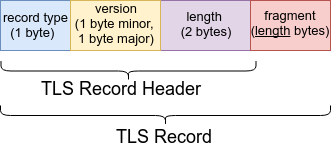
\includegraphics[width=0.6\textwidth]{img/record-header-3.png} % first figure itself
  \caption{\label{fig:tls-record-header} TLS Record header}
\end{figure}

\begin{figure}
\centering
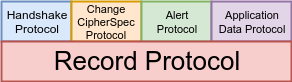
\includegraphics[width=0.6\textwidth]{img/tls-sub-protocols-3.png} % second figure itself
\caption{\label{fig:tls-subprotocols} TLS (Sub)protocols and Layers}
\end{figure}

\subsection{TLS 1.2 Handshake Protocol} \label{hsp}

The Handshake Protocol is responsible for negotiating a \textbf{session},
which will then be used in a \textbf{connection}.
There is a difference between a \gls{tls} session and a \gls{tls} connection:
\begin{itemize}
  \item \textbf{TLS session} - association between two communication peers that is
  created by the \textbf{TLS Handshake Protocol}, which defines a set of negotiated parameters
  (cryptographic and others, such as
  the compression algorithm, depending on the \gls{tls} version) that are used by the \textbf{TLS connections associated
  with that session}. A single \textbf{TLS session} can be shared among multiple
  \textbf{TLS connections} and its main purpose is to avoid the expensive negotiation
  of new parameters for each \textbf{TLS connection}. For example, let us say
  that a \gls{html} page is being downloaded over the \gls{https} and that page references some images from that same server using \gls{https} links. Instead of the web browser negotiating a new \gls{tls} session for every single image again, it can re-use the the
  one it has established to download the \gls{html} page,
  saving time and computational resources. Session resumption can be done using various
  approaches, such as \textbf{session identifiers}, described throughout \codeword{Section 7.4}
  of \codeword{RFC 5246}\cite{RFC5246} and \textbf{session tickets}, defined in
  \codeword{RFC 5077}\cite{RFC5077}.
  \item \textbf{TLS connection} - used to actually transmit the cryptographically
  protected data. For the data to be cryptographically protected, some parameters,
  such as the secret keys used to encrypt and authenticate the transmitted
  data need to be established; this is done when a \textbf{TLS session} is created,
  during the \textbf{TLS Handshake Protocol}.
\end{itemize}

\begin{figure}
        \centering
        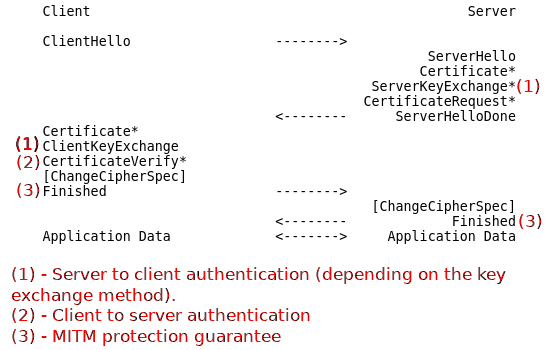
\includegraphics[width=0.9\textwidth]{img/tls-12-full-handshake2.png} % first figure itself
        \caption{\label{fig:tls-12-handshake} \gls{tls} $1.2$ message flow for a full handshake}
\end{figure}

\begin{figure}
  \centering
  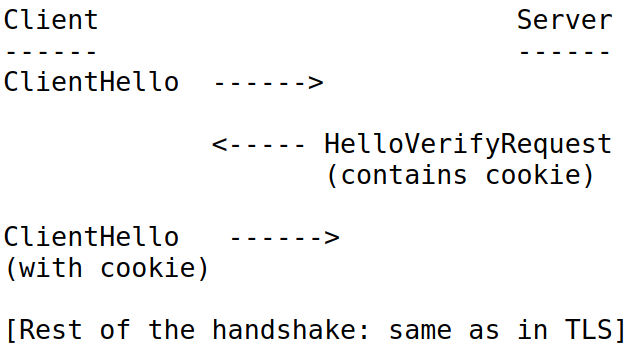
\includegraphics[width=0.6\textwidth]{img/dtls-cookie.png} % second figure itself
  \caption{\label{fig:dtls-cookie} DTLS handshake with HelloVerifyRequest containing the cookie}
\end{figure}


In the handshake phase the client and the server agree on which version of the \gls{tls}
protocol to use, authenticate one to another and negotiate session state items like
the cipher suite and the compression method.  Figure \ref{fig:tls-12-handshake} shows the message flow for the
full \gls{tls} $1.2$ handshake. \codeword{*} indicates situation-dependent
messages that are not always sent. \codeword{ChangeCiperSpec} is a separate
protocol, rather than a message type.

As already mentioned, every \gls{tls} handshake message is encapsulated within
a \gls{tls} record. The actual handshake message is contained within the
\codeword{fragment} of a \gls{tls} record. The record type for a handshake
message is \codeword{0x16}. The handshake message has the following structure:
a 1-byte \codeword{msg_type} field (specifies the Handshake message type),
a 2-byte \codeword{length} field (specifies the length of the \codeword{body})
and a \codeword{body} field, which contains a structure depending on the
\codeword{msg_type} (similar to \codeword{fragment} field in a \gls{tls} record).

A typical handshake message flow will be described next, with only the most important fields of each message mentioned.

The \gls{tls} handshake starts with the client sending a \codeword{ClientHello}, containing \codeword{random}, \codeword{cipher_suites} and \codeword{compressison_methods},
among other fields.
\\\codeword{cipher_suites} contains a \textbf{list} of cipher suites and \codeword{compression_methods}
contains a \textbf{list} of compression methods that the
client supports, \textbf{ordered by preference}, with the most preferred one appearing first.
The \gls{tls} record contains a $2$-byte \codeword{version} field which
indicates the highest version supported by the client.

The server responds to the \codeword{ClientHello} with a \codeword{ServeHello}.
This message is similar, but contains the chosen \codeword{cipher_suite}
and \codeword{compression_method} from the list sent by the client. Just like in the client's case, a \codeword{random}
is present. The \codeword{version} field in the \gls{tls} record indicates
the \gls{tls} version chosen by the server, which will be the one used for
that connection.

\gls{tls} requires cryptographically secure pseudorandom numbers to be generated
by both of the parties independently. Those random numbers (or \textit{nonces}) are essential for freshness
(protection against replay attacks) and session uniqueness. To provide those
properties, both of the random values are required. Those two random values are inputs to the \gls{prf} when the master secret is generated, meaning
that a new keying material will be obtained with every new session. If the output of the pseudorandom number generator
can be predicted by the attacker, he can predict the keying material, as described
in "A Systematic Analysis of the Juniper Dual EC Incident"\cite{DualECJu15:online}.
The \codeword{32-byte} random value is composed by concatenating the \codeword{4-byte}
GMT UNIX time with \codeword{28} cryptographically random bytes. Note that, in \gls{tls} $1.3$,
the random number structure has the same length, but is generated in a different manner:
the client's \codeword{32 bytes} are all random, while the server's last \codeword{8 bytes}
are fixed when negotiating \gls{tls} $1.2$ or $1.3$.

Next, the server sends a \codeword{Certificate} message, which contains a list
of public key certificates: the server's certificate,
every intermediate certificate and the root certificate, \textit{i.e}, a certificate chain. The certificate's contents
will depend on the negotiated cipher suite and extensions.
The same message type occurs later in the handshake, if the server requests the client's certificate with the
\codeword{CertificateRequest} message. In a typical scenario, the
server will not request client authentication.

The \codeword{ServerKeyExchange} message follows, containing additional information
needed by the client to compute the premaster secret. This message
is only sent in some key exchange methods, namely \codeword{DHE_DSS}, \codeword{DHE_RSA}
and \codeword{DH_anon}. For non-anonymous key exchanges, this is the message that authenticates the server to the client,
since the server sends a digital signature over the client and server randoms, as well as the server's key exchange parameters. Note that this is not the only place where the
server can authenticate itself to the client. For example, if \codeword{RSA} key
exchange is used, the server authentication is done indirectly when the client
sends the premaster secret encrypted with the public \gls{rsa} key provided in the
server certificate. Since only the server knows the corresponding private key, if
both of the sides generate the same keying material, then the server must be who
it claims to be. In \gls{tls} $1.3$ this message is non-existent and a similar
functionality is taken by the \codeword{key_exchange} extension.

The \codeword{ServerHelloDone} is sent to indicate the end of \codeword{ServerHello}
and associated messages. Upon the receipt of this message, the client should check
if the server provided a valid certificate. This message is not present in \gls{tls} 1.3.

With the \codeword{ClientKeyExchange} message the premaster secret is
set. This is done either by direct transmission of the secret generated by the client
and encrypted with the server's public \gls{rsa} key (thus, authenticating the server to the client)
or by the transmission of \gls{dh} parameters that will allow each side to generate
the same premaster secret independently. In \gls{tls} $1.3$ this message is
non-existent and a similar functionality is taken by the
\codeword{key_exchange} extension.

The \codeword{CertificateVerify} message is sent by the client to verify its
certificate. This message is only sent if client authentication is used and
if the client's certificate has signing capability (\textit{i.e.} all certificates except for the ones
containing fixed \gls{dh} parameters).

The \codeword{ChangeCipherSpec} is its own protocol, rather than a type of handshake
message. It is sent by both parties to notify the receiver that subsequent records
will be protected under the newly negotiated \codeword{cipher spec} and keys.
This message is not present in \gls{tls} $1.3$.

The \codeword{Finished} message is an essential part of the protocol. It is the first
message protected with the newly negotiated algorithms, keys and secrets. Only after
both parties have sent and verified the contents of this message they can
be sure that the Handshake has not been tampered with by a \gls{mitm} and begin to
receive and send application data. Essentially, this message contains a keyed hash
with the master secret over the hash of all the data from all of the
handshake messages not including any \codeword{HelloRequest} messages and up to, but
not including, this message. The other party must perform the same computation on its
side and make sure that the result is identical to the contents of the other party's
\codeword{Finished} message. If at some point a \gls{mitm} has tampered with the
handshake, there will be a mismatch between the computed and the received contents of the
\codeword{Finished} message.

At any time after a session has been negotiated, the server may send a \codeword{HelloRequest}
message, to which the client should respond with a \codeword{ClientHello}, thus
beginning the negotiation process anew.

At any point in the handshake, the Alert protocol may be used by any of the peers
to signal any problems or even abort the process through the use of an appropriate message type.

Besides the full handshake, \gls{tls} $1.2$ also defines an
abbreviated handshake mechanism, which can be used to either resume a previous session,
or duplicate one, instead of negotiating new security parameters. This
requires state to be maintained by both peers. The advantage of this mechanism is that the handshake is reduced
to \codeword{1 RTT}, instead of the usual \codeword{2 RTT}, as it is the case in the full handshake.

In order to perform an abbreviated handshake,
the client and the server must have established a session previously, by the
means of a full handshake. In its \codeword{ServerHello} phase, the server generates and sends a \codeword{session_id}, which will be associated with the newly negotiated session.

To resume a session, in its \codeword{ClientHello} phase the client includes the \codeword{session_id} of the session it wants to
resume. It is up to the server to decide if it
will resume that session. In the positive case, the server responds with a \codeword{ServerHello} containing
the same \codeword{session_id} value as the one sent by the client. In the negative
case, the \codeword{ServerHello} will contain a different \codeword{session_id} value, thus
triggering a new session negotiation process.

The keying material, such as the bulk
data symmetric encryption keys and the \gls{mac} keys are formed by hashing the new client
and server random values with the master secret. Therefore, provided that the master secret has not been compromised and that the secure
hash operations are, in fact, secure, the new connection will be secure and independent
from previous ones. The \gls{tls} $1.2$ spec, suggests and upper limit
of $24$ hours for \codeword{session ID} lifetimes, since an attacker which obtains the master secret
may be able to impersonate the compromised party until the corresponding \codeword{session ID} is retired.

\subsection{\gls{tls} Record Processing} \label{record}

A \gls{tls} record must go through some processing before it can be sent over the network.
This processing is done by the \textbf {TLS Record Protocol} and involves the following steps (\codeword{1-4} for \gls{tls} $1.2$ and \codeword{1, 3-4} for \gls{tls} $1.3$):

\begin{enumerate}
  \item \textbf{Fragmentation} - the \textbf{TLS Record Layer} takes arbitrary-length data and \textbf{fragments}
  it into manageable pieces: each one of the resulting fragments is called a \codeword{TLSPlaintext}.
  Client message boundaries are not preserved, which means that multiple messages
  of the same type may be placed into the same fragment or a single message may
  be fragmented across several records.
  \item  \textbf{Compression} (removed in \gls{tls} 1.3) - the \textbf{TLS Record Layer} compresses the
  \codeword{TLSPlaintext} structure according to the negotiated compression method,
  outputting \codeword{TLSCompressed}. Compression is optional. If the negotiated compression
  method is \codeword{null}, \codeword{TLSCompressed} is identical to \codeword{TLSPlaintext}.
  \item \textbf{Cryptographic Protection} - in \gls{tls} 1.2, either an
  \gls{aead} cipher or a separate encryption and \gls{mac} functions transform a
  \codeword{TLSCompressed} fragment into a \codeword{TLSCipherText} fragment. In the case
  of \gls{tls} 1.3, the \codeword{TLSPlaintext} fragment is transformed into a \codeword{TLSCipherText} by applying an \gls{aead} cipher, since all
  non-\gls{aead} ciphers have been removed.
  \item Append the \codeword{TLS Record Header} - encapsulate \codeword{TLSCipherText}
  in a \codeword{TLS Record}.
\end{enumerate}

\begin{figure}
  \centering
  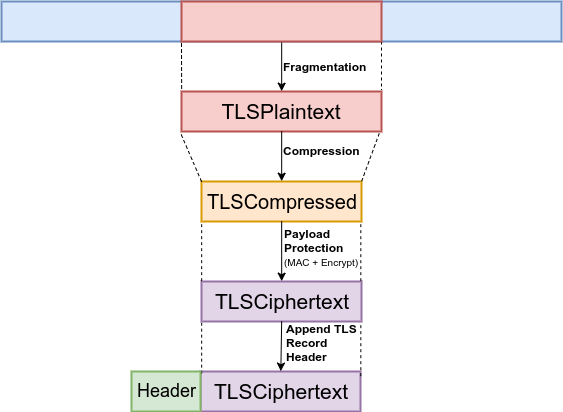
\includegraphics[width=1.0\textwidth]{img/tls-record-processing-3.png}
  \caption{\label{fig:tls-record-processing}TLS 1.2 Record Processing}
\end{figure}

The process described above, as well as the structure names are depicted in Figure \ref{fig:tls-record-processing}.
The compression step is not present in \gls{tls} 1.3. The structure names are exactly as the appear in the \gls{tls} specifications.

\subsection{\gls{tls} Keying Material} \label{keying}

In \gls{tls}, the confidentiality and integrity guarantees are achieved through the use
of \gls{sc}. Consequently, the communicating peers need to \textbf{share}
a \textbf{set of keys}. In \gls{tls} they are derived independently by the
client and the server, during the \gls{tls} Handshake Protocol.

The keys appear with different names in \gls{tls} $1.2$ and $1.3$ specs, but
they serve the same purpose. Additionally, more more keys can be found in
\gls{tls} $1.3$, for reasons that will be covered in Section \ref{tls-13}.
In \gls{tls} 1.2, the peers agree on the following set of keys:

\begin{itemize}
  \item \codeword{client write key} - used by the client to encrypt the data to be sent
  \item \codeword{client read_key} - used by the client to decrypt the incoming data from the server
  \item \codeword{server write key} - used by the server to encrypt the data to be sent
  \item \codeword{server read key} - used by the server to decrypt the incoming data from the server
  \item \codeword{client write IV} - used by the client for implicit nonce techniques with \gls{aead} ciphers
  \item \codeword{server_write_IV} - used by the server for implicit nonce techniques with \gls{aead} ciphers
  \item \codeword{client write MAC key} (\gls{tls} 1.2 only) - used by the client to authenticate the data to be sent
  \item \codeword{client write MAC key} (\gls{tls} 1.2 only) - used by the client to authenticate the data to be sent
\end{itemize}

When communicating with one another, the client uses one key to
encrypt the data that it sends to the server and another key, different from the first one, to decrypt the data
that it receives from the server, and vice-versa. This implies that the  following relationships must hold:
\codeword{client write key == server read key} and \codeword{server write key == client read key}.

\subsection{TLS 1.2 Keying Material Generation} \label{keying-material}

The generation of secret keys, used for various cryptographic operations involves the
following steps, in order:

\begin{enumerate}
  \item Generate the \textbf{premaster secret}.
  \item From the \textbf{premaster secret} generate the \textbf{master secret}.
  \item From the \textbf{master secret} generate the various secret keys, which
  will be used in the cryptographic operations.
\end{enumerate}

The derivation of the keying material needed for a connection is done using
the \gls{tls} \gls{prf}. It is defined as \codeword{PRF(secret, label, seed) = P_hash(secret, label + seed)}.
The \codeword{P_hash(secret, seed)} function is an auxiliary data expansion function
which uses a single cryptographic hash function to expand a \codeword{secret} and a \codeword{seed}
into an arbitrary quantity of output. Therefore, it can be used to generate
anywhere from $1$ to an infinite number of bits of output. \codeword{PRF(secret, label, seed)}
is used to generate as many bits of output as needed. When generating the
master secret, the \codeword{secret} input is the \codeword{premaster secret}.
When generating the key block, from which the final keys will be obtained,
the \codeword{secret} input is the \codeword{master secret}.

The cryptographic hash function used in \codeword{P_hash(secret, label, seed)} is
the hash function that is implicitly defined by the cipher suite in use. All of the cipher
suites defined in the \gls{tls} $1.2$ base spec use \codeword{SHA-256} and any new
cipher suites must explicitly specify a the same hash function or a stronger one.

\subsection{TLS 1.2 Key Exchange Methods} \label{key-exchange}

The way the peremaster secret is generated depends on the key exchange
method used. This is the only phase of the keying material generation
phase that is variable for a fixed cipher suite, since a cipher suite defines
the \gls{prf} function that will be employed. Neither the derivation of the
shared keys are impacted by the key exchange method.

There are many key exchange methods to choose from. Some of them
are defined in the base spec (\codeword{RFC5246}\cite{RFC5246}), while others
in separate \gls{rfc}s. For example, the \gls{ecc} based key exchange, specified
in \codeword{RFC4492} \cite{RFC4492}).

The base spec specifies four key exchange methods, one using \gls{rsa} and
three using \gls{dh}:

\begin{itemize}
  \item static \gls{rsa} (\codeword{RSA}; removed in \gls{tls} 1.3) - the client generates the premaster secret, encrypts it with the
  server's public key (which it obtained from the server's \codeword{X.509} certificate) and
  sends it to the server. The server then decrypts it using the corresponding private key and uses it as its premaster secret. \gls{pfs} is
  a property that preserves the confidentiality of past interactions even if the
  long-term secret is compromised. This key exchange method offers authenticity, but does not offer \gls{pfs}.
  \item anonymous \gls{dh} (\codeword{DH_annon}; removed in \gls{tls} 1.3) -
  each run of the protocol, uses
  different pubic \gls{dh} parameters, which are generated dynamically. This results
  in a different, \textbf{ephemeral} key being generated every time. Since the exchanged \gls{dh}
  parameters are \textbf{not authenticated}, the resulting key exchange
  vulnerable to \gls{mitm} attacks. \gls{tls} $1.2$ spec states that cipher suites
  using \codeword{DH_annon} \textbf{must not} be used, unless the application
  layer explicitly requests so. This key exchange offers \gls{pfs}, but does not offer
  authenticity.
  \item fixed/static \gls{dh} (\codeword{DH}; removed in \gls{tls} 1.3) - the server's/client's public \gls{dh} parameter
  is embedded in its certificate. This key exchange method offers authenticity,
  but does not offer \gls{pfs}.
  \item ephemeral \gls{dh} (\codeword{DHE}) - the \gls{dh} protocol is used, identically to \codeword{DH_annon}, but the public parameters
  are digitally signed in some way, usually using the sender's private
  \gls{rsa} (\codeword{DHE_RSA}) or \gls{dsa} (\codeword{DHE_DSS}) key. This key
  exchange offers both, authenticity and \gls{pfs}.
\end{itemize}

When either of the \gls{dh} variants is used, the value obtained from the exchange is used
as the premaster secret. Usually, only the server's
authenticity is desired, but client's can also be achieved if it supplies the
server with its certificate. Whenever the server is authenticated, it is secure
against \gls{mitm} attacks. Table \ref{kemsp} summarizes the security properties
offered by each key exchange method.

\begin{table}[]
\centering
\caption{Key exchange methods and security properties}
\label{kemsp}
\begin{tabular}{|l|c|l|}
\hline
\textbf{Key Exch Meth} & \multicolumn{1}{l|}{Authentication} & PFS                    \\ \hline
RSA                          & X                                   &                        \\ \hline
DH\_anon                     & \multicolumn{1}{l|}{}               & \multicolumn{1}{c|}{X} \\ \hline
DH                           & X                                   &                        \\ \hline
DHE                          & X                                   & \multicolumn{1}{c|}{X} \\ \hline
\end{tabular}
\end{table}

In \gls{tls} $1.3$, static \gls{rsa} and \gls{dh} ciphersuites have been removed, meaning that all
public key exchange mechanisms now provide \gls{pfs}. Even though
anonymous \gls{dh} key exchange has been removed,
unauthenticated connections are still possible, by either using raw public keys\cite{RFC7250} or not verifying the certificate chain and any of its contents.

The use of \gls{ecc}-based key exchange (\gls{ecdh} and \gls{ecdhe}) and authentication (\gls{ecdsa})
algorithms with \gls{tls} is described in \codeword{RFC4492}\cite{RFC4492}. The document introduces five new
\gls{ecc}-based key exchange algorithms, all of which use \gls{ecc} to compute
the premaster secret, differing only in whether the negotiated
keys are ephemeral (\gls{ecdh}) or long-term (\gls{ecdhe}), as well as the mechanism (if any) used to
authenticate them. Three new \gls{ecdsa} \textbf{client authentication} mechanisms are also defined,
differing in the algorithms that the certificate must be signed with, as well
as the key exchange algorithms that they can be used with.
Those features are negotiated through \gls{tls} extensions.

\subsection{TLS Extensions} \label{extensions}

\gls{tls} extensions were originally defined in \codeword{RFC 4366}\cite{RFC4366}
and later merged into the \gls{tls} $1.2$ base spec. Each extension consists of an
extension type, which identifies the particular extension type, and extension data,
which contains information specific to a particular extension.

The extension mechanism can be used by \gls{tls} clients and servers; it is backwards
compatible, which means that the communication is possible between a \gls{tls} client that supports a particular extension and a server that does not support it,
and vice versa. A client may request the use of extensions by sending an extended \codeword{ClientHello}
message, which is just a "normal" \codeword{ClientHello} with an additional
block of data that contains a list of extensions. The backwards compatibility is achieved based on the \gls{tls}
requirement that the servers that are not "extensions-aware" must ignore the data
added to the \codeword{ClientHello}s that they do not understand (section \codeword{7.4.1.2} of \codeword{RFC 2246}\cite{RFC2246}). Consequently,
even servers running older \gls{tls} versions that do not support extensions, will not "break".

The presence of extensions can be determined by checking if there are bytes
following the \codeword{compression_methods} field in the \codeword{ClientHello}.
If the server understands an extension, it sends back an extended \codeword{ServerHello},
instead of a regular one. An extended \codeword{ServerHello} is a regular
\codeword{ServerHello} with an additional block of data following the
\codeword{compression_method}, containing a list of extensions.

An extended \codeword{ServerHello} message can only be sent in a response to an
extended \codeword{ClientHello} message. This prevents the possibility that an extended
\codeword{ServerHello} message could cause a malfunction of older \gls{tls} clients that do not
support extensions. An extension type must not appear in the
extended \codeword{ServerHello}, unless the same extension type appeared in the
corresponding extended \codeword{CleintHello}, and if this happens, the client must abort the handshake.

\subsection{TLS 1.3} \label{tls-13}

Due to limited space, \gls{tls} $1.3$\cite{I-D.ietf-tls-tls13} will not be described in detail. The focus was on \gls{tls} $1.2$ instead, because \gls{tls} $1.3$ is still in draft
mode and $1.2$ is the latest and the recommended to use version.
Despite the protocol name not suggesting it, \gls{tls} $1.3$ is
very different from \gls{tls} 1.2. It should have probably been called
\gls{tls} $2.0$ instead.

Numerous differences from \gls{tls} $1.3$ to $1.2$ have been mentioned throughout the document.
Various characteristics found in \gls{tls} $1.3$ make it more suitable for the context
of \gls{iot} than \gls{tls} $1.2$. Some of them were already mentioned previously, and in this section a additional ones will be outlined.

The first important difference is that the use of extensions is required in \gls{tls} $1.3$.
This can be explained by the fact that some of the functionality has been moved into extensions, in order to preserve
backwards-compatibility with the \codeword{ClientHello}s of the previous versions.
The way a server distinguishes if a client is requesting \gls{tls} $1.3$
is by checking the presence of the \codeword{supported_versions} extension in the
extended \codeword{ClientHello}.

In \gls{tls} $1.3$ more data is encrypted and the encryption begins earlier. For example,
at the server-side there is a notion of "encrypted extensions". The \codeword{EncryptedExtensions}
message, as the name suggests, contains a list of extensions that are encrypted
under a symmetric key. It contains any extensions that are not needed
for the establishment of the cryptographic context.

One of the main problems with using \gls{tls} in \gls{iot} is that while \gls{iot}
traffic needs to be quick and lightweight, \gls{tls} $1.2$ adds two additional
round trips (\codeword{2 RTT}) to the start of every session. \gls{tls} $1.3$ handshake has a lower latency,
and this is extremely important in the context of \gls{iot}.
The full \gls{tls} $1.3$ handshake is only \codeword{1 RTT}. \gls{tls} $1.3$ even allows
clients to send data on the first flight (known as \textbf{early client data}), when the clients
and servers share a \gls{psk} (either obtained externally or via a previous handshake).
This means that in \gls{tls} $1.3$ \codeword{0-RTT} data is possible, by
encrypting it with a key derived from a \gls{psk}. Session resumption
via identifiers and tickets has been obsoleted in \gls{tls} $1.3$, and both methods
have been replaced by a \gls{psk} mode. This \gls{psk} is established in a previous
connection after the handshake is completed and can be presented by the client
on the next visit.

Keying material generation is more complex in \gls{tls} $1.3$ than in
\gls{tls} $1.2$, since different
keys are used to encrypt data throughout the Handshake protocol. This can be
explained by the fact that in \gls{tls} $1.3$ the encryption begins earlier.
Other Handshake messages besides \codeword{Finished} are encrypted. As a result,
multiple encryption keys are generated and used to encrypt different data
throughout the handshake.

The way the keying material is derived is also different. The
\gls{prf} construction described above has been replaced.
In \gls{tls} 1.3, key derivation uses the
\gls{hkdf} function \cite{RFC5869} and its two components: \codeword{HKDF-Extract} and \codeword{HKDF-Expand}.
This new design allows easier analysis by cryptographers due to improved
key separation properties.

%
\subsection{\gls{dtls}} \label{dtls}

As already mentioned, \gls{dtls} is an adaption of \gls{tls} that runs on
top of an unreliable transport protocol, such as UDP. The design of \gls{dtls} is deliberately very similar to \gls{tls}, in fact, its specification is written
in terms of differences from \gls{tls}. This similarity allows to
both, minimize new security invention, and maximize the amount of code and infrastructure reuse. The changes are mostly done at the lower level and
don not affect the core of the protocol.
Even extensions defined before \gls{dtls} existed can be
used with it. The latest version of \gls{dtls} is $1.2$ and it is defined
in \codeword{RFC 6347}\cite{RFC6347}. There is a draft of \gls{dtls} $1.3$
\cite{I-D.ietf-tls-dtls13} that is currently under active development.

Since \gls{dtls} operates on top of an unreliable transport protocol, such as
UDP, it must explicitly deal with the absence of reliable and ordered assumptions
that are made by \gls{tls}. The main differences from \gls{dtls} $1.2$ to \gls{tls} $1.2$ are:

\begin{itemize}
  \item two new fields are added to the record layer: an explicit \codeword{2 byte} sequence
  number and a \codeword{6 byte} epoch. The \gls{dtls} \gls{mac} is the same as in \gls{tls},
  however, rather than using the implicit sequence number, the \codeword{8 byte} value
  formed by concatenation of the epoch number and the sequence number is used.

  \item stream ciphers must not be used with \gls{dtls}.

  \item a stateless cookie exchange mechanism has been added to the handshake protocol
  in order to prevent \gls{dos} attacks. To accomplish this, a new handshake
  message, the \codeword{HelloVerifyRequest} has been added. After
  the \codeword{ClientHello}, the server responds with a \codeword{HelloVerifyRequest}
  containing a cookie, which is returned back to the server in another
  \codeword{ClientHello} that follows it. After this, the handshake proceeds as in \gls{tls}. This is depicted in Figure \ref{fig:dtls-cookie}.   Although optional for the server, this mechanism highly recommended, and the
  client must be prepared to respond to it. \gls{dtls} $1.3$ follows the same idea, but does it differently, namely,
  the \codeword{HelloVerifyRequest} message has been removed, and the cookie is conveyed to the client via an extension in a \codeword{HelloRetryRequest} message.

  \item the handshake message format has been extended to deal with message reordering,
  fragmentation and loss by addition of three new fields: a message sequence field,
  a fragment offset field and a fragment length field.
\end{itemize}

\section{Related Work}

Lightweight cryptography is an important topic in the context of \gls{iot} security, due to the resource-limited nature of the devices. This section will begin with the description of the work done in this area.

Biryukov \textit{et al}\cite{Stateoft96:online} explore the topic of lightweight symmetric cryptography,
providing a summary of the lightweight symmetric
primitives from the academic community, the government agencies and even proprietary
algorithms which have been either reverse-engineered or leaked. All of those algorithms
are listed in the paper, alongside relevant metrics. The list will not be
included herein due to the lack of space. The authors also proposed
to split the field into two areas: ultra-lightweight and \gls{iot} cryptography.

The paper systematizes the knowledge in the area oe lightweight cryptography
in order to define "lightweightness" more precisely. The authors observed that the design
of lightweight cryptography algorithms varies greatly, the only unifying thread
between them being the low computing power of the devices that they are designed for.

The most frequently optimized metrics are the memory consumption, the implementation size
and the speed or the throughput of the primitive. The specifics depend on whether
the hardware or the software implementations of the primitives are considered.

If the primitive is implemented in hardware, the memory consumption and the implementation
size are lumped together into its gate area, which is measured in Gate Equivalents (GE),
a metric quantifying how physically large a circuit implementing the primitive is.
The throughout is measured in \textit{bytes/sec} and it corresponds to the amount of plaintext
processed per time unit. If a primitive is implemented in software (typically for
use in micro-controllers), the relevant metrics are the RAM consumption, the code
size and the throughput of the primitive, measured in \textit{bytes/CPU cycle}.

To accommodate the limitations of the constrained devices, most lightweight algorithms
are designed to use smaller internal states with smaller key sizes. After analysis,
the authors concluded that even though at least \codeword{128 bit} block and
key sizes were required from the AES candidates, most of the lightweight
block ciphers used only \codeword{64-bit} blocks, which leads to a smaller memory
footprint in both, software and hardware, while also making the algorithm better suited
for processing of smaller messages.

Even though algorithms can be optimized in implementation: whether it is
a software or a hardware, dedicated lightweight algorithms are still needed.
This comes down mainly to two factors: there are limitations to the the extent of
the optimizations that can be done and the hardware-accelerated encryption is
frequently vulnerable to various \gls{sca}s. An example of such an attack is the one done on the
Phillips light bulbs \cite{cryptoeprint:2016:1047}, where the authors were able to
recover a secret key used to authenticate updates.

It is more difficult to implement a lightweight hash function than a lightweight
block cipher, since standard hash functions need large amounts
of memory to store both: their internal states, for example, \codeword{1600 bits} in case of SHA-3,
and the block they are operating on, for example, \codeword{512 bits} in the case of SHA-2.
The required internal state is acceptable for a desktop computer, but not for a
constrained device. Taking this into consideration, the most common approach
taken by the designers is to use a sponge construction with a very small bitrate.
A sponge function is an algorithm with an internal state that takes as an input
a bit stream of any length and outputs a bit stream of any desired length. Sponge
functions are used to implement many cryptographic primitives, such as cryptographic
hashes. The bitrate decides how fast the plain text is processed and how fast the
final digest is produced. A smaller bitrate means that the output will take longer
to be produced, which means that a smaller capacity (the security level)
can be used, which minimizes the memory footprint at the cost of slower data
processing. A capacity of \codeword{128 bits} and a bitrate of \codeword{8 bits}
are common values for lightweight hash functions.

Another trend in the lightweight algorithms noticed by the authors is the
preference for \textit{ARX}-based and \textit{bitsliced-S-Box} based designs, as well as simple key schedules.

Finally, a separation of the "lightweight algorithm" definition into two distinct fields has been proposed:

\begin{itemize}
  \item \textbf{Ultra-Lightweight Crypto} - algorithms running on very cheap
  devices \textbf{not connected to the internet}, which are easily replaceable
  and have a limited life-time. Examples: \textit{RFID} tags, smart cards and remote car keys.
  \item \textbf{IoT Crypto} - algorithms running on a low-power device,
  \textbf{connected to a global network}, such as the internet. Examples: security cameras, smart light bulbs and smart watches.
\end{itemize}

Considering the two definitions above, this the work of this dissertation focuses on \textbf{IoT Crypto}
devices. A summary of differences between the both categories is summarized in
table \ref{ul-iot}.

\begin{table}[]
\centering
\caption{A summary of the differences between ultra-lightweight and IoT crypto}
\label{ul-iot}
\begin{tabular}{@{}lll@{}}
\toprule
                           & \textbf{Ultra-Lightweight}          & \textbf{IoT}                           \\ \midrule
\textbf{Block Size}        & 64 bits                             & ≥ 128 bits                             \\
\textbf{Security Level}    & ≥ 80 bits                           & ≥ 128 bits                             \\
\textbf{Relevant Attacks}  & low data/time complexity            & same as "regular" crypto               \\
\textbf{Intended Platform} & dedicated circuit (ASIC, RFID...)   & micro-controllers, low-end CPUs        \\
\textbf{SCA Resilience}    & important                           & important                              \\
\textbf{Functionality}     & one per device, e.g. authentication & encryption, authentication, hashing... \\
\textbf{Connection}        & temporary, only to a given hub      & permanent, to a global network         \\ \bottomrule
\end{tabular}
\end{table}

While there is a high demand for lightweight public key primitives, the required
resources for them are much higher than for symmetric ones. As a
paper by Katagi \textit{et al}\cite{b5b8db9716:online}
concluded, there are no promising primitives
that have enough lightweight and security properties, compared to the
conventional ones, such as RSA and \gls{ecc}. Further research on this topic, as part of the work on this dissertation, lead to the same conclusion.

Lightweight cryptography is an important topic this work and there are papers detailing
various algorithms. In order to provide a good overview of it while staying succinct, recent papers that provide a summary of the
area, rather than focusing on specific implementations, were chosen.
The remainder of this section will focus on the work done on the (D)\gls{tls} protocol in the context of \gls{iot}.

The "Scalable Security With Symmetric Keys"\cite{S3KScala62:online} paper proposes a key management architecture for resource-constrained devices,
which allows devices that have no previous, direct security relation to use
(D)\gls{tls} using one of two approaches: shared symmetric keys or raw public keys.
The resource-constrained device is a server that offers one or more resources,
such as temperature readings. The idea in both approaches is to introduce a third-party
\codeword{trust anchor (TA)} that both, the client and the server use to establish
trust relationships between them.

The first approach is similar to Kerberos\cite{RFC4120}, and it does not require any
changes to the original protocol. A client can request a \gls{psk} \codeword{Kc} from the \codeword{TA},
which will generate it and send it back to the client via a secure channel, alongside
a \codeword{psk_identity} which has the same meaning and use as in \codeword{RFC 4279}\cite{RFC4279}. When connecting to the server,
the client will send to the server the \codeword{psk_identity} that it received in a previous
handshake. Upon its receipt, the server will derive the \codeword{Kc}, using the
\codeword{P_hash()} function defined in \codeword{RFC 5246}\cite{RFC5246}.

The second approach consists in requesting an \gls{apk}
from the \codeword{TA}. The client includes his \gls{rpk} in its request, which is used for authorization. The TA
creates an authorization certificate, protects it with a \gls{mac} and sends it
to the client alongside the server's public key.
The client then sends this \gls{apk} (instead of the \gls{rpk})
when connecting to the server, which verifies it (to authorize the client)
and proceeds with the handshake in the \gls{rpk} mode, as defined in \codeword{RFC 4279} \cite{RFC4279}.
To achieve this, a new certificate structure is defined, alongside a new \codeword{certificate_type}.
The new certificate structure is just the \codeword{RFC7250} \cite{RFC7250} structure, with an
additional \gls{mac}.

The hash function used for key derivation is SHA256. The authors evaluated the
performance of their solution with and without SHA2 hardware acceleration and
concluded that while it had significant impact on key derivation, it had little
impact on the total handshake time (\codeword{711.11 ms} instead of \codeword{775.05 ms}), since most of the time was spent in sending
data over the network and other parts of the handshake, the longest one being
the \codeword{ChangeCipherSpec} message which required a processing time
of \codeword{17.79ms}.

6LoWPAN\cite{RFC4944} is a protocol that allows devices with limited processing
ability and power to transmit information wirelessly using the \codeword{IPv6}
protocol. The protocol defines IP Header Compression (IPHC) for the IP header, as well as,
Next Header Compression (NHC) for the IP extension headers and the UDP header in \codeword{RFC 6282}\cite{RFC6282}.
The compression relies on the shared context between the communicating peers.

The work proposed in \cite{6LoWPANC53:online} uses this same idea, but with the goal of compressing \gls{dtls} headers.
6LoWPAN does not provide ways to compress the UDP payload and layers above.
A proposed standard\cite{RFC7400} for generic header compression
for 6LoWPANs that can be used to compress the UDP payload, does exit, however. The authors propose
a way to compress \gls{dtls} headers and messages using this mechanism.

Their work defines how the \gls{dtls} Record header, the \gls{dtls} Handshake header,
the \codeword{ClientHello} and the \codeword{ServerHello} messages can be compressed, but notes that
the same compression techniques can be used to compress the remaining handshake
messages. They explore two cases for the header compression: compressing both,
the Record header and the Handshake header and compressing the Record header only,
which is useful after the handshake has completed and the fragment field of the
Record layer contains application data, instead of a handshake message.


\begin{figure}
  \centering
  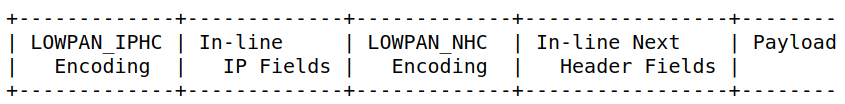
\includegraphics[width=0.9\textwidth]{img/6lowpan-header.png} % first figure itself
  \caption{\label{fig:6lowpan-header} IPv6 Next Header Compression}
\end{figure}

\begin{figure}
  \centering
  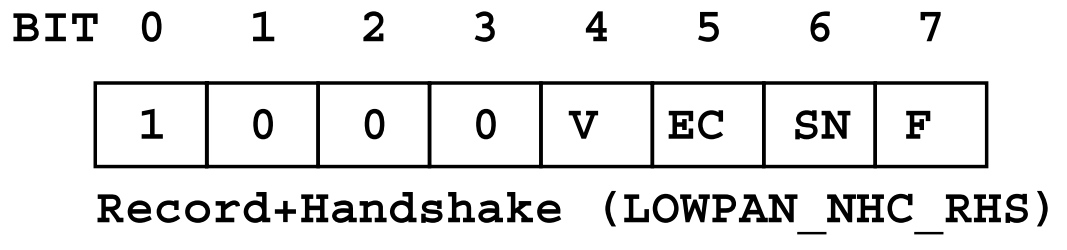
\includegraphics[width=0.6\textwidth]{img/6lowpan-ghc-rhs.png} % second figure itself
  \caption{\label{fig:6lowpan-ghc-rhs} LOWPAN\_NHC\_RHS structure}
\end{figure}


Each \gls{dtls} fragment is carried over as a UDP payload. In this case,
the UDP payload carries a header-like payload (the \gls{dtls} record header).
Figure \ref{fig:6lowpan-header} shows the way IPv6 next header compression is done.
The authors use the same value for the \codeword{LOWPAN_NHC Encoding} field (defined in \codeword{RFC 6282}\cite{RFC6282})
as in \codeword{RFC7400} and define the format of the \codeword{In-line Next Header Fields}
(also defined in \cite{RFC6282}), which is the compressed \gls{dtls} content. The \codeword{LOWPAN_IPHC Encoding}
and \codeword{In-Line IP Fields} fields are used in the IPv6 header compression
and are not in the scope of the paper.

All of the cases follow the same basic idea, for this reason only one of them will be exemplified:
the case where both, the Record and the Handshake headers are compressed.
In this case \codeword{LOWPAN_NHC Encoding} will contain the \codeword{LOWPAN_NHC_RHS}
structure (depicted in figure \ref{fig:6lowpan-ghc-rhs}), which is the compressed form of the Record and Handshake headers. The
parts that are not compressed will be contained in the \codeword{Payload} part.
The first four bits represent the ID field and in this case they are fixed to \codeword{1000},
that way, the decompressor knows what is being compressed (\textit{i.e} how to interpret
the structure that follows the ID bits). If the \codeword{F} field of the \codeword{LOWPAN_NHC_RHS} structure contains the
bit \codeword{0}, it means that the handshake message is not fragmented, so
the \codeword{fragment_offset} and \codeword{fragment_length} fields are
elided from the Handshake header (common case when a handshake message is not bigger than
the maximum header size), meaning that they are not going to be sent at
all (\textit{i.e.} they are not going to be present in the \codeword{Payload} part).
If the \codeword{F} bit has the value \codeword{1}, the \codeword{fragment_offset}
and \codeword{fragment_length} fields are carried inline (\textit{i.e.} they are
present in the \codeword{Payload} part). The remaining two fields define similar
behavior for other header fields (some of them assume that some default value is present, when a field is elided).
The \codeword{length} field in the Record and Handshake headers are always elided,
since they can be inferred from the lower layers.

The evaluation showed that the compression can save a significant number of bits:
the Record header, that is included in all messages can be compressed by \codeword{64 bits}
(\textit{i.e.} by $62\%$).

There is also a proposal for TCP header compression for 6LoWPAN\cite{I-D.aayadi-6lowpan-tcphc},
which if adopted, in many cases can compress the mandatory \codeword{20 bytes} TCP header
into \codeword{6 bytes}. This means that the same ideas can be applied to TCP and
\gls{tls} as well.

Later, in 2013, Raza \textit{et al.} proposed a security scheme called Lithe\cite{LitheLig40:online},
which is a lightweight security solution for \gls{coap} that uses the same \gls{dtls} header
compression technique as in \cite{6LoWPANC53:online} with the goal of implementing
it as a security support for \gls{coap}. \gls{coap}\cite{RFC7959} is a specialized
\textit{REST}ful Internet Application Protocol for constrained devices. it is designed to easily
translate to HTTP, in order to simplify its integration with the web,
while also meeting requirements such as multicast support and low overhead.
\gls{coap} is like "HTTP for constrained devices".
It can run on most devices that support UDP or a UDP-like protocol.
\gls{coap} mandates the use of \gls{dtls} as the underlying security protocol for
authenticated and confidential communication. There is also a \gls{coap} specification
running on top of TCP, which uses \gls{tls} as its underlying security protocol
currently being developed\cite{I-D.ietf-core-coap-tcp-tls}.

The authors evaluated their system in a simulated environment in \textit{Contiki OS}\cite{ContikiT75:online}, which is an open-source operating system for the \gls{iot}.
They obtained significant gains in terms of packet size (similar numbers to the
ones observed in \cite{6LoWPANC53:online}), energy consumption (on average $15\%$ less
energy is used to transmit and receive compressed packets), processing time
(the compression and decompression time of \gls{dtls} headers is almost negligible)
and network-wide response times (up to $50\%$ smaller RTT). The
gains in the mentioned measures are the largest when the compression avoids
fragmentation (in the paper, for payload size of \codeword{48 bytes}).

Angelo \textit{et al.} \cite{Security5:online} proposed to integrate the \gls{dtls} protocol
inside \gls{coap}, while also exploiting \gls{ecc} optimizations and minimizing
ROM occupancy. They implemented their solution in an off-the-shelf mote platform
and evaluated its performance. \gls{dtls} was designed to protect web application communication, as a result,
it has a big overhead in \gls{iot} scenarios. Besides that, it runs over UDP,
so additional mechanisms are needed to provide the reliability and ordering
guarantee. With this in mind, the authors wanted to design a version of \gls{dtls}
that both: minimizes the code size and the number of exchanged messages, resulting
in an optimized Handshake protocol.

In order to minimize the code size occupied by the \gls{dtls} implementation, they
decided to delegate the tasks of \textbf{reliability} and \textbf{fragmentation} to
\gls{coap}. This means that the code responsible for those functionalities,
can be removed altogether from the \gls{dtls} implementation, thus reducing ROM
occupancy. This part of their work was based on an informational RFC draft\cite{I-D.keoh-dtls-profile-iot}, in which the
authors profiled \gls{dtls} for \gls{coap}-based \gls{iot} applications and proposed
the use of a \textit{RESTful} \gls{dtls} handshake which relies on \gls{coap} block-wise
transfer to address the fragmentation issue.

To achieve this they  proposed the use of a \textit{RESTful} \gls{dtls} connection as a \gls{coap} resource,
which is created when a new secure session is requested.
The authors exploit the the \gls{coap}s capability to provide connection-oriented
communication offered by its message layer. In particular, each \codeword{Confirmable}
\gls{coap} message requires an \codeword{Acknowledgement} message (page 8 of \codeword{RFC 7252} \cite{RFC7252}),
which acknowledges that a specific \codeword{Confirmable} message has arrived, thus
providing reliable retransmission.

Instead of leaving the fragmentation function to \gls{dtls}, it was
delegated to the block-wise transfer feature of \gls{coap}\cite{RFC7959}, which was developed
to support transmission of large payloads. This approach has two advantages: first, the code in the \gls{dtls}
layer responsible for this function can be removed, thus reducing ROM occupancy,
and second, the fragmentation/reassembly process burdens the lower layers
with state that is better managed in the application layer.

The authors also optimized the implementation of basic operations on which
many security protocols, such as \gls{ecdh} and \gls{ecdsa} rely upon. The first
optimization had to do with modular arithmetic on large integers. A set of optimized
assembly routines based on \cite{Comparin25:Online} allow the improved use of
registers, reducing the number of memory operations needed to perform
tasks such as multiplications and square roots on devices with \codeword{8-bit} registers.

Scalar multiplication is often the most expensive operation in \gls{ec}-based
cryptography, therefore optimizing it is of high interest. The authors used a
technique called \textit{IBPV} described in \cite{LowcostS87:online}, which is based on pre-computation.
of a set of discrete log pairs. The mathematical details have been purposefully omitted,
since they are not relevant for this description. The \textit{IBPV} technique was used
to improve the performance of the \gls{ecdsa} signature and extended to the
\gls{ecdh} protocol. In order to reduce the time taken to perform an \gls{ecdsa}
signature verification, the \textit{Shamir Trick} was used, which allows
to perform the sum of two scalar multiplications (frequent operation in \gls{ec} cryptography)
faster than performing two independent scalar multiplications.

The results showed that the \gls{ecc} optimizations
outperform the scalar multiplication in the state of the art class 1 device platforms,
while also improving the the network lifetime by a factor of up to $6.5$ with
respect to a standard, non-optimized implementation. Leaving reliability and
fragmentation tasks to \gls{coap}, reduces the \gls{dtls} implementation code size
by approximately $23\%$.

\codeword{RFC 7925}\cite{RFC7925} describes a \gls{tls} and \gls{dtls} $1.2$
profile for \gls{iot} devices that offer communication security services
for \gls{iot} applications.
In this context, "profile" means available configuration options (ex: which
cipher suites to use) and protocol extensions that are best suited for \gls{iot} devices.
The document is rather lengthy, only its fundamental parts will be summarized. A number of relevant \gls{rfc}s will also be described.

\codeword{RFC 7925} explores both cases: constrained clients and constrained servers, specifying
a profile for each one and describing the main challenges faced in each scenario.
The profile specifications for constrained clients and servers are very similar.
Code reuse in order to minimize the implementation size is recommended. For example, an \gls{iot} device
using a network access solution based on \gls{tls}, such as EAP-TLS\cite{rfc5216}
can reuse most parts of the code for (D)\gls{dtls} at the application layer.

For the credential types the profile considers 3 cases:

\begin{itemize}
  \item \gls{psk} - authentication based on \gls{psk}s is described in
  \codeword{RFC 4249}\cite{RFC4279}. When using \gls{psk}s, the client indicates which
  key it wants to use by including a \gls{psk} identity in its \codeword{ClientKeyExchange} message.
  A server can have different \gls{psk} identities shared with different clients.
  An identity can have any size, up to a maximum of \codeword{128 bytes}.
  The profile recommends the use of shorter \gls{psk} identities and specifies
  \codeword{TLS_PSK_WITH_AES_128_CCM_8} as the only mandatory-to-implement
  cipher suite to be used with \gls{psk}s, just like \gls{coap} does. If a \gls{pfs} cipher suite is used, ephemeral
  \gls{dh} keys should not be reused over multiple protocol exchanges.

  \item \gls{rpk} - the use of \gls{rpk}s in (D)\gls{tls} is described in \codeword{RFC 7250}\cite{RFC7250}.
  With \gls{rpk}s, only a subset of the information that is found in typical certificates
  is used: namely the \codeword{SubjectPublicKeyInfo} structure, which contains
  the necessary parameters to describe the public key (the algorithm identifier
  and the public key itself). Other PKIX certificate\cite{RFCabc} parameters are
  omitted, making the resulted \gls{rpk} smaller in size, when compared to the
  original certificate and the code to process the keys simpler. In order for the
  peers to negotiate a \gls{rpk}, two new extensions have been defined:
  one for the client indicate which certificate types it can provide to the server, and one to indicate which certificate types it can process from the server. To further reduce the size of the implementation, the profile
  recommends the use of the \gls{tls} Cached Information extension\cite{RFC7924}, which
  enables \gls{tls} peers to exchange just the fingerprint (a shorter sequence of bytes
  used to identify a public key) of the public key. Identical to \gls{coap}, the only mandatory-to-implement
  cipher suite to be used with \gls{rpk}s is \codeword{TLS_ECDHE_ECDSA_WITH_AES_128_CCM_8}.

  \item certificate - conventional certificates can also be used. The support
  for the Cached Information extension\cite{RFC7924} and the\\ \codeword{TLS_ECDHE_ECDSA_WITH_AES_128_CCM_8}
  cipher suite is required. The profile restricts the use of named curves to
  the ones defined in \codeword{RFC 4492}\cite{RFC4492}. For certificate revocation, neither the
  \gls{ocsp}\cite{RFC6960}, nor the \gls{crl}\cite{RFCabc} mechanisms are used, instead this task is delegated to
  the software update functionality. The Cached Information extension does not
  provide any help with caching client certificates. For this reason, in cases
  where client-side certificates are used and the server is not constrained,
  the support for client certificate URLs is required. The client certificates URL
  extension\cite{RFC4366} allows the clients to point the server to a URL from
  which it can obtain its certificate, which allows constrained clients to
  save memory and amount of transmitted data. The Trusted CA Indication\cite{RFC6066}
  extension allows the clients to indicate which trust anchors they support, which is useful
  for constrained clients that due to memory limitation posses only a small number
  of \gls{ca} root keys, since it can avoid repeated handshake failures. If the clients interacts with
  dynamically discovered set of (D)\gls{tls} servers, the use of this extension is recommended,
  if that set is fixed, it is not.

\end{itemize}

The signature algorithms extension\cite{RFC5246} allows the client to indicate
to the server which signature/hash pairs it supports to be used with digital signatures.
The client must send this extension to indicate the use of \codeword{SHA-256},
otherwise the defaults defined in \cite{RFC5246} are used. This extension is not
applicable when \gls{psk}-based cipher suites are used.

The profile mandates that constrained clients must implement session
resumption to improve the performance of the handshake since this will lead to
less exchanged messages, lower computational overhead (since only symmetric cryptography
is used) and it requires less bandwidth. If server is constrained, but
the client is not, the client must implement the Session Resumption Without
Server-Side State mechanism\cite{RFC5077}, which is achieved through the
use of tickets. The server encapsulates the state into a ticket and forwards it to
the client, which can subsequently resume the session by sending back that ticket.
If both, the client and the server are constrained, both of them should implement
\codeword{RFC 5077}\cite{RFC5077}.

The use of compression is not recommended for two reasons. First, \codeword{RFC7525}\cite{RFC7525}
recommends disabling (D)\gls{tls} level compression, due to attacks such as \codeword{CRIME}\cite{Microsof72:online}.
\codeword{RFC7525} provides recommendations for improving the security of deployed services
that use \gls{tls} and \gls{dtls} and was published as a response to the various
attacks on (D)\gls{tls} that have emerged over the years. Second, for \gls{iot} applications,
the (D)\gls{tls} compression is not needed, since application-layer protocols are highly
optimized and compression at the (D)\gls{tls} layer increases the implementation's size and complexity.

\codeword{RFC6520}\cite{RFC6520} defines a heartbeat mechanism to test whether the peer
is still alive. The implementation of this extension is recommended for server
initiated messages. Note that since the messages sent to the client will most likely
get blocked by middleboxes, the initial connection setup is initiated by the
client and then kept alive by the server.

Random numbers play an essential role in the overall security of the protocol.
Many of the usual sources of entropy, such as the timing of keystrokes and the
mouse movements, will not be available on many \gls{iot} devices, which means that
either alternative ones need to be found or dedicated hardware must be added.
\gls{iot} devices using (D)\gls{tls} must find ways to offer to the generation of quality
random numbers, the guidelines and requirements for which can be found in \codeword{RFC4086}\cite{rfc4086}.

Implementations compliant with the profile must use \gls{aead} ciphers, therefore
encryption and \gls{mac} computation are no longer independent steps, which means
that neither encrypt-then-MAC\cite{RFC7366}, nor the truncated MAC\cite{RFC6066} extensions are applicable
to this specification and must not be used.

The \gls{sni} extension\cite{RFC6066} defines a mechanism for a client to
tell a (D)\gls{tls} server the name of the server that it is contacting. This is
crucial in case when multiple websites are hosted under the same IP address.
The implementation of this extension is required, unless the (D)\gls{tls}
client does not interact with a server in a hosting environment.

The maximum fragment length extension\cite{RFC6066} lowers the maximum fragment
length support of the record layer from $2^14$ to $2^9$. This extension allows
the client to indicate the server how much of the incoming data it is able to buffer,
allowing the client implementations to lower their RAM requirements, since it does not
not need to accept packets of large size, such as the \codeword{16K} packets required by
plain (D)\gls{tls}. For that reason, client implementations must support this
extension.

The Session Hash Extended Master Secret Extension\cite{RFC7627} defines an extension
that binds the master secret to the log of the full handshake, thus preventing
\gls{mitm} attacks, such as the triple handshake\cite{TripleHa89:online}. Even though the
cipher suites recommended by the profile are not vulnerable to this attack, the
implementation of this extension is advised. In order to prevent the renegotiation
attack\cite{RFC5746}, the profile requires the \gls{tls} renegotiation feature
to be disabled.

With regards to the key size recommendations, the authors recommend symmetric keys
of at least \codeword{112 bit}, which corresponds to a \codeword{233-bit} \gls{ecc}
key and to a \codeword{2048} \gls{dh} key. Those recommendations are made
conservatively under the assumption that \gls{iot} devices have a long expected
lifetime ($10+$ years) and that those key recommendations refer to the long-term
keys used for device authentication. Keys that are provisioned dynamically
and used for protection of transactional data, such as the ones used in
(D)\gls{tls} cipher suites, may be shorter, depending on the sensitivity of
transmitted data.

Even though \gls{tls} defines a single stream cipher: \textit{RC4}, its use is no longer
recommended due to its cryptographic weaknesses described in \codeword{RFC 7465}\cite{RFC7465}.

\codeword{RFC 7925}\cite{RFC7925} points out that designing a software
update mechanism into an \gls{iot} system is crucial to ensure that potential vulnerabilities
can be fixed and that the functionality can be enhanced. The software update mechanism
is important to change configuration information, such as trust anchors and
other secret-key related information. Although the profile refers to \codeword{LM2M}\cite{OpenMobi29:online}
as an example of protocol that comes with a suitable software update mechanism,
there has been new work done in this area since the release of this profile.
There is a document specifying an architecture for a firmware update
mechanism for \gls{iot} devices\cite{I-D.moran-suit-architecture} currently in Internet-Draft state.

\section{Solution}

\subsection{Solution Architecture}

Most of the work has been centered around \gls{dtls},
even though the majority of solutions can be applied to \gls{tls} as well.
Herein we want to explore \gls{tls} optimization more. There is clearly a need for that, specially with \gls{coap} over
TCP and \gls{tls} standard being currently developed. The mentioned standard does not explore any \gls{tls}
optimizations, and since any \gls{iot} device using it in the future would benefit from
them, this is an important area to explore. None of the related work explored
(D)\gls{tls} 1.3, mainly because the protocol is still in draft stages, however, major design changes are not expected at this point.

The majority of the work done in the area proposes a solution that is either tied to a
specific protocol, such as \gls{coap}, or requires an introduction of a third-party
entity, such as the trust anchor in the case of the S3K system\cite{S3KScala62:online} or
even both. This two main issues. First, a protocol-specific solution can not
be easily used in an environment where (D)\gls{tls} is not used with that protocol. Second, the requirement of a third-party
introduces additional cost and complexity, which will be a big resistance factor
in adopting the technology. This is specially true for developers working on
personal projects or projects for small businesses, leaving the communications insecure
in the worse case scenario. The goal of this work is to design a solution that can be used out
of the box and is not tailored towards any specific protocol, while fully backwards
compatible with the original protocol, that can be used with either \gls{tls}
or \gls{dtls} and would work with both versions: (D)\gls{tls} $1.2$ and the upcoming
(D)\gls{tls} 1.3.

In order to achieve those goals, the \gls{tls} extension
mechanism will be heavily relied upon. By using extensions, any deviations from the original protocol can be done, even if they completely change it. This was confirmed by
one of the \gls{tls} designers, after we asked this question on the official
\gls{ietf} mailing list\cite{ReTLSTLS31:online}, since neither of the existing \gls{rfc}s made it clear.

Ideas from \gls{tls} $1.3$, such as \codeword{0-RTT data}, which can be done if peers already share a \gls{psk} would be interesting to
explore for (D)\gls{tls} $1.2$.
For example, this can be very useful in the context of the temperature sensor
described in the introduction, where the device sends data to a server every
30 seconds. With \codeword{0-RTT data}, it can communicate securely with minimal costs.
The use of symmetric cryptography exclusively, has various advantages in the context
of \gls{iot}. This means that there is value in exploring solutions that revolve around
\gls{psk}s and that avoid public key cryptography completely.

Not all \gls{iot} devices are limited to the point of not being able to use
public key cryptography altogether. For some of them, the use of \gls{rpk}s, which is considered the first entry point into the area of public key
cryptography, is acceptable, while others are powerful enough to take
advantage of certificates and \gls{pki}, at least up to a point.
The solution proposed with this work
would be adaptable to any of those scenarios, depending on the context and the security
requirements, therefore being similar to a framework. For example, some scenarios
might require integrity, but not privacy. For those, it does not make sense to
pay the energy and time overhead of encryption. Special care in the
selection of cipher suites and key exchange methods needs to be taken, possibly even developing new ones.

(D)\gls{tls} $1.2$ is significantly different from (D)\gls{tls} 1.3
and there has been no work like \codeword{RFC 7924}\cite{RFC7924}, which describes a lightweight (D)\gls{tls} profile, done for (D)\gls{tls} $1.3$.
This is an important topic to explore. (D)\gls{tls} $1.3$ has many fundamental changes
to the way the handshake is done, bringing many new features, whose ideas can
be incorporated into the proposed solution and even backported to \gls{tls} 1.2.

% src: https://tex.stackexchange.com/questions/5769/two-figures-side-by-side
\begin{figure}
    \centering
    \begin{minipage}{0.5\textwidth}
        \centering
        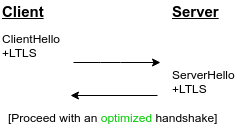
\includegraphics[width=1.0\textwidth]{img/optimized-handshake.png} % first figure itself
        \caption{\label{fig:ltls-opt} LTLS supported}
    \end{minipage}\hfill
    \begin{minipage}{0.5\textwidth}
        \centering
        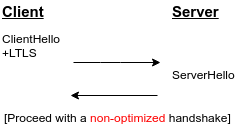
\includegraphics[width=1.0\textwidth]{img/non-optimized-handshake.png} % second figure itself
        \caption{\label{fig:ltls-non-opt} LTLS not supported}
    \end{minipage}
\end{figure}

To exemplify the idea of the solution, let us assume that a
Lightweight TLS (LTLS) extension is defined. The optimizations that will be described in the second part of this work will be incorporated into it. Let us consider the case of a client that wants to use those
optimizations. To achieve this, it will include the LTLS extension in its
\codeword{ClientHello}. If the server supports the extension, an
optimized connection can be established; this case is depicted in Figure \ref{fig:ltls-opt}. If the server does not support the extension, it will not
send it back in its \codeword{ServerHello}. In that case it is possible
to fall back to regular (D)\gls{tls}, as depicted in Figure \ref{fig:ltls-non-opt}.

In practice the extension will include additional data used to indicate various options, which has been omitted from the discussion for simplicity.

\subsection{Evaluation}

In order to evaluate the quality of the work, both, the original protocol
implementation and the one provided as part of the solution, will be profiled and compared. The relevant profiling metrics are power consumption, RAM usage, storage usage,
CPU cycles elapsed and time taken. The profiling
will be done over various simulated scenarios, which emulate real-life usage,
such as connecting to the server multiple times over a short time period and transferring
small quantities of data, and connecting to the server and transferring a large
amount of data, all at once.

Due to limited time and the fact that \gls{tls} $1.3$ still lacks stable implementations, most likely, only the solution under \gls{tls} $1.2$ will be implemented and evaluated.

\subsection{Planning}

During the month of February, up until mid-March $2018$, the solution will be defined precisely.
Due to the nature of the solution, it will have many different versions, depending
on the target device and required security services. Most likely, there will be no time
to implement and evaluate every possible scenario, so only a subset of them will be chosen.

From mid-March until mid-April $2018$, a version that uses existing configuration options and protocol extensions to best support the
\gls{iot} environment will be developed. In essence, this would involve incorporating a lightweight profile (like \codeword{RFC 7925} does) into the solution. The system will be implemented in code, by modifying
the \textit{mbedTLS 2.6.0} library\cite{SSLLibra13:online}.

From mid-April until June $2018$, the customized part will be implemented.
This might involve custom cipher suites, key exchange methods and changes in
the Handshake Protocol.

From June until July $2018$, the work will be concentrated around \gls{psk}
solutions. This might involve adapting the existing \gls{psk} configurations
or creating new ones.

From July until August $2018$, the work will be evaluated. The most important
evaluation metrics will be chosen and the related profiling code set up. Testing
scenarios will be designed and implemented.

From mid-July until mid-September $2018$, the focus will be on writing the
dissertation's text. Some minor improvements and additions might also be done
during this period of time.

\section{Conclusion}

The lack of security in \gls{iot} is a serious issue that can lead to a high monetary costs,
when botnets infect the devices. Recent
attacks clearly show that serious damage can be caused. An old saying attributed to the
\gls{nsa} states that "Attacks always get better; they never get worse".
Combined with the fact that the number of \gls{iot} devices is growing at a high
pace, without any major improvements to their security, makes it clear
that it is fundamental for this issue to be addressed.

While there are well established security solutions, not all of them can be used
with \gls{iot} devices, due their constrained nature. One such example is
the (D)\gls{tls} protocol, that because of its heavyweight nature is not suitable for a large part of \gls{iot} devices. With future work,
we want to contribute to this area, by designing a solution that is suitable for the \gls{iot} devices, transparent
to the programmer and has the provided security services adaptable to the specific context needs.

% ---- Bibliography ----
%
\nocite{*}
\bibliographystyle{unsrt}
\bibliography{tls_for_iot,papers}
%
\printglossary[style=long]
%
\end{document}
